\documentclass[letter,10pt]{article}
\usepackage{amsfonts}
\usepackage{amsmath}
\usepackage[font=small,labelfont=bf]{caption}
\usepackage{fancyhdr}
\usepackage[margin=1.0in]{geometry}
\usepackage{graphicx}
\usepackage{hyperref}
\usepackage{multicol}
\usepackage{textcomp}
 %
\setlength{\columnsep}{0.5cm}
\pagestyle{fancy}
\fancyhf{}
\lhead{
	CSE 847: Machine Learning---Project Proposal \\
	Langford, Lingg, and Lucero
}
\rhead{February 17, 2017}
\cfoot{\thepage}
\begin{document}
	\title{
		CSE 847: Machine Learning---Project Proposal \\
		\textbf{An Exploration and Implementation of Automated Valuation Models to Learn and Predict the Value of Real Estate}
	}
	\author{
		\begin{tabular}{ccc}
			Mick Langford & Mike Lingg  & Jordi Lucero \\
			langfo37@msu.edu & linggmic@egr.msu.edu & luceroj2@msu.edu
		\end{tabular}
	}
	\date{February 17, 2017}
	\maketitle
	\begin{multicols}{2}
		\section{Problem Description}
		Automated Valuation Models (AVM) have become increasingly popular as the real estate market has embraced the World Wide Web as a source of accurate, up to the minute data.\textsuperscript{\cite{kaggleblog}} Banks have also shown great interest in using AVMs to help mitigate fraud by human appraisal.\textsuperscript{\cite{scotsman}} Our goal is to explore various machine learning techniques to implement an AVM and predict the true value of a house based on features commonly found on real estate listings.  Our data will be drawn from the Nashville, TN housing market, using a dataset posted on Kaggle\textsuperscript{\cite{nashville_data}}.
		\par
		We will begin by exploring linear regression models that take into account physical attributes of each house and location. Further work will be performed exploring nonlinear models, such as deep learning with neural networks and decision trees, which can be compared and contrasted. Additional work may be performed to explore missing feature estimation.
		\section{Related Work}
		An obvious and popular example is Zillow's proprietary Zestimate\textsuperscript{\textregistered}. Zillow uses a closed source AVM that takes into account special features of the home, location, and market conditions. Zillow admits to using features such as physical attributes, tax assessments, and prior transactions. Zillow claims to have data on 110 million homes and estimates on approximately 100 million homes.\textsuperscript{\cite{zillow}}
		\par
		Relevant papers include the doctoral dissertation of Lowrance which explores and compares various linear models on housing data for the Los Angeles County.\textsuperscript{\cite{lowrance}} Park and Bae explore machine learning algorithms such as C4.5, RIPPER, Naive Bayesian, and AdaBoost.\textsuperscript{\cite{park}} Bin performed a study that estimates a hedonic price function using a semi-parametric regression.\textsuperscript{\cite{bin}} This may be particularly useful for real estate listings that are incomplete or for data that is entered erroneously. Bourassa et al. consider the spatial dependence of house prices, which is intuitively an important factor.\textsuperscript{\cite{bourassa1}\cite{bourassa2}} Kauko et al. research neural network models to help investigate segmentation in the housing market of Helsinki, Finland.\textsuperscript{\cite{kauko}} Azadeh et al. present an algorithm based on fuzzy linear regression and a fuzzy cognitive map to handle uncertainty in the housing market and improve the analysis of housing price fluctuations.\textsuperscript{\cite{azadeh}} Fan et al. introduce a decision tree approach for modeling and predicting house prices.\textsuperscript{\cite{fan}}
		\section{Project Data}
		For this project we are working with multiple data sources pulled from real housing sales data.
		\par
		\textbf{Nashville Housing Data} The Nashville housing data set is a list of home sales in the Nashville, Tennessee area, provided by Kaggle\textsuperscript{\cite{nashville_data}}.  This data set includes 29 fields of data for 56635 entries. However, nearly half of the entries have gaps in information, which will have to be accounted for. We further augmented this data set by using an geocoding service provided by the United State Census Bureau to add the zip code, latitude, and longitude for entries where a match could be found.
		\par
		\textbf{King County Housing Data} The King County housing data set is a list of home sales in the King County, Washington area, provided by Kaggle\textsuperscript{\cite{kc_data}}. This data set includes 20 fields of data for 21614 entries, with none of the entries missing any data.
		\par
		\textbf{Advanced Regression Techniques Data} The Advanced Regression Techniques data is a list of home sales, provided by Kaggle. This data includes 79 features of housing data for 1460 homes. The data has no gaps, except for some N/A data.
		\par
		\textbf{Redfin Data} The Redfin data is a list of home sales in the Grand Rapids area, provided by Redfin. This data includes 14 fields for 9646 entries. The data set also has gaps in information for about half of the entries.
		\par
		The different data sets provide a variety of input to test machine learning techniques against. Data with more features should provide more accurate results. One challenge will be to determine the best way to manage entries with missing information. Two methods are being considered. The first method is to simply substitute missing values with their associated mean values. Another method is to consider the values that are present for each entry, find the nearest neighboring entry, by way of Euclidean distance, and substitute the missing values with that neighbor's values.
		\par
		For pre-processing the data, we will be normalizing the data set, by dividing each feature value by the difference between that feature's maximum and minimum values. Another problem being considered is how to properly manage fields containing categorical values. Our approach will be to treat a field with \(n\) categories as \(n\) binary features, indicating whether that entry is of the associated category or not.
		\section{Project Progress}
		Figure \ref{fig:ganttchart} shows our initial project milestones and timeline to completing them.
	\end{multicols}
	\begin{figure*}[t]
	    \centering
	    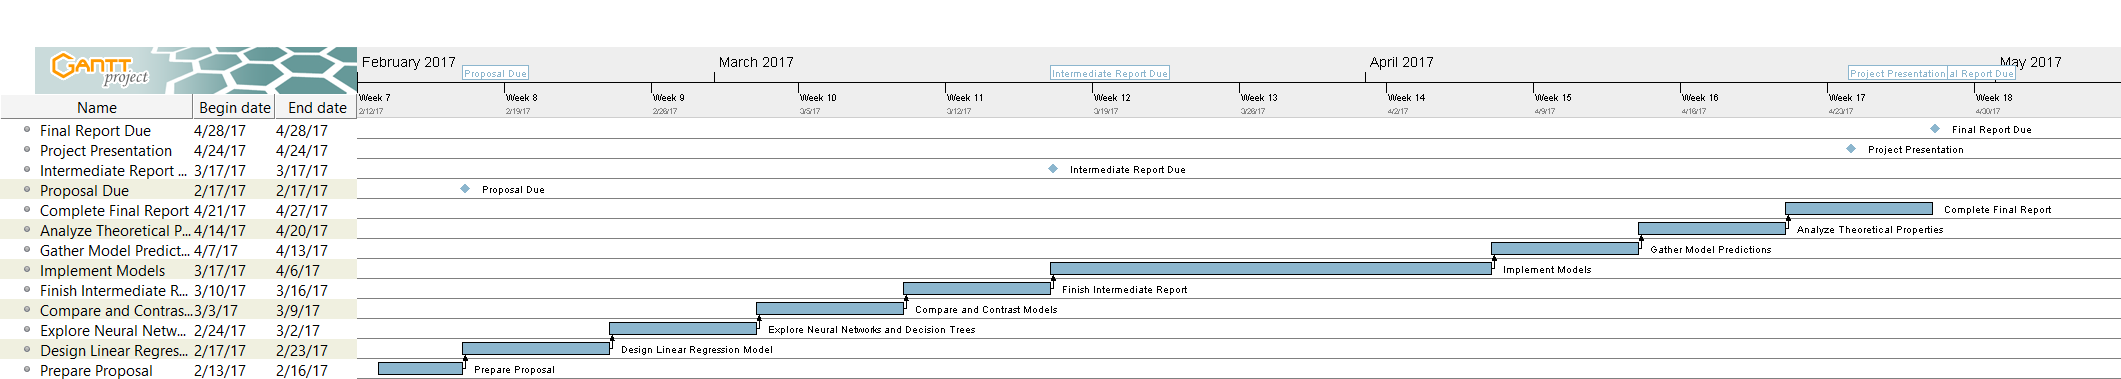
\includegraphics[width=\textwidth]{Schedule/ProjectSchedule.png}
	    \caption{Gantt Chart showing  our project milestones and expected completion dates.}
	    \label{fig:ganttchart}
	\end{figure*}
	\begin{multicols}{2}
		\subsection{Linear Regression}
		Initial work has been done on developing working linear regression models.  These models include a closed, form ridge regression model, a standard linear descent model and a stoicastic linear descent model.  All three models perform roughly the same, with a mean squared error is better than the results of MATLAB's built in fitlm function.  One interesting behavior noted is that the highest accuracy is achieved at lower house values, where the highest density of data points is sitting.  Additional work is planned to try to eliminate the few large error points, perhaps by seeing if this is caused by a bad feature.
		\subsection{Logistic Regression}
		Two working logistic regression models have been created.  Both models separate the houses into categories by value.  The categories start at the lowest value house and put all homes in the same \$ 5k range into a category.  The first model creates a set of model weights for each category and places a house in the category producing the highest logistic regression result.  The second model creates a a set of model weights that categorize each house price as being higher or lower than the current category, then for each category the house price is higher for, the estimated value is increased by 5k.
		\subsection{Decision Tree}
		\subsection{Neural Network}
		\subsection{Additional Work}
		In addition to the existing models having been developed, we are considering creating a Support Vector Machine model to categorize house prices by features.
		?? Model compare and contrast?

		\begin{thebibliography}{13}
			\bibitem{nashville_data}
			\textit{Nashville Housing Data: Home value data for the booming Nashville Market}
			Retrieved from \\ \small{\url{https://www.kaggle.com/tmthyjames/nashville-housing-data/}}
			
			\bibitem{kc_data}
			\textit{House Sales in King County, USA: Predict house price using regression}
			Retrieved from \\ \small{\url{https://www.kaggle.com/harlfoxem/housesalesprediction}}	
			
			\bibitem{kaggleblog}
			\textit{Data-driven property valuations: the real deal?}
			Retrieved from \\ \small{\url{http://blog.kaggle.com/2010/06/21/data-inc-are-avms-soothsayers-or-the-real-deal/}}
			
			\bibitem{scotsman}
			Schroeder, Steve.
			\textit{Fighting Fraud: A combination of collateral assessment and AVMs can maximize mortgage-fraud management}
			Retrieved from \\ \small{\url{http://www.scotsmanguide.com/Residential/Articles/2005/10/Fighting-Fraud/}}
			
			\bibitem{zillow}
			\textit{What is a Zestimate? Zillow's Home Value Forecast.}
			Retrieved from \\
			\small{\url{http://www.zillow.com/zestimate/}}
			
			\bibitem{lowrance}
			Lowrance, R. E. (2015).
			\textit{Predicting the Market Value of Single-Family Residential Real Estate}
			(Doctoral Dissertation). New York University. Retrieved from \small{\url{http://gradworks.umi.com/36/85/3685886.html}}
			
			\bibitem{park}
			Park, B., \& Bae, J. K. (2015).
			\textit{Using machine learning algorithms for housing price prediction: The case of Fairfax County, Virginia housing data.}
			Expert Systems with Applications, 42(6), 2928-2934. doi:10.1016/j.eswa.2014.11.040
			
			\bibitem{bin} 
			Bin, O. (2004).
			\textit{A prediction comparison of housing sales prices by parametric versus semi-parametric regressions.}
			Journal of Housing Economics, 13(1), 68-84. doi:10.1016/j.jhe.2004.01.001
			
			\bibitem{bourassa1} 
			Bourassa, S. C., Cantoni, E., \& Hoesli, M. (2010). 
			\textit{Predicting House Prices with Spatial Dependence: Impacts of Alternative Submarket Definitions.}
			SSRN Electronic Journal. doi:10.2139/ssrn.1090147
			
			\bibitem{bourassa2}
			Bourassa, S. C., Cantoni, E., \& Hoesli, M. (2007).
			\textit{Spatial Dependence, Housing Submarkets, and House Prices.}
			SSRN Electronic Journal. doi:10.2139/ssrn.771867
			
			\bibitem{kauko}
			Kauko, T., Hooimeijer, P., \& Hakfoort, J. (2002).
			\textit{Capturing Housing Market Segmentation: An Alternative Approach based on Neural Network Modelling.}
			Housing Studies, 17(6), 875-894. doi:10.1080/02673030215999
			
			\bibitem{azadeh} 
			Azadeh, A., Ziaei, B., \& Moghaddam, M. (2012).
			\textit{A hybrid fuzzy regression-fuzzy cognitive map algorithm for forecasting and optimization of housing market fluctuations.}
			Expert Systems with Applications, 39(1), 298-315. doi:10.1016/j.eswa.2011.07.020
			
			\bibitem{fan}
			Fan, G., Ong, S. E., \& Koh, H. C. (2006).
			\textit{Determinants of House Price: A Decision Tree Approach.}
			Urban Studies, 43(12), 2301-2315. doi:10.1080/00420980600990928
		\end{thebibliography}
	\end{multicols}
\end{document}